\documentclass{jsarticle}

\usepackage{amsmath}
\usepackage{amssymb}
\usepackage{booktabs}
\usepackage{float}
\usepackage{graphicx}
\usepackage{listings}
\usepackage{url}

\lstset{
  basicstyle={\ttfamily},
  identifierstyle={\small},
  commentstyle={\smallitshape},
  keywordstyle={\small\bfseries},
  ndkeywordstyle={\small},
  stringstyle={\small\ttfamily},
  frame={tb},
  breaklines=true,
  columns=[l]{fullflexible},
  numbers=left,
  xrightmargin=0zw,
  xleftmargin=3zw,
  numberstyle={\scriptsize},
  stepnumber=1,
  numbersep=1zw,
  lineskip=-0.5ex
}

\title{情報領域演習第二 L演習(クラス3) レポート}
\author{学籍番号: 1810678 \\
        名前: 山田朔也}

\begin{document}
  \maketitle
  \begin{description}
      \item[問1.]
      \begin{description}
          \item[(a)]
          まず、与えられた論理式$f$の否定$\overline{f}$を計算し、それを積和標準形に変形する。その後、積和標準形で表された論理式$\overline{f}$のさらに否定$\overline{\overline{f}}$を計算することで、和積標準形に変換することができる。これらの計算は全てド・モルガンの法則を適用し、分配律に沿って計算することで求めることが可能である。

          \item[(b)]
          \begin{description}
              \item[$\rm \hspace{.18em}i\hspace{.18em}$.]
              まず、与えられた論理式$f_1$の否定$\overline{f_1}$を計算する
              \begin{align}
                  \overline{f_1} &= \overline{(x\overline{y}\overline{z} + \overline{x}y\overline{z} +  \overline{x}\overline{y}z)} \notag \\
                                 &= \overline{(x\overline{y}\overline{z})} \cdot \overline{(\overline{x}y\overline{z})} \cdot \overline{(\overline{x}\overline{y}z)} \notag \\
                                 &= (\overline{x}+y+z) \cdot (x+\overline{y}+z) \cdot (x+y+\overline{z}) \notag \\
                                 &= \overline{x}\overline{y}\overline{z} + \overline{x}yz + xyz + xy\overline{z} + x\overline{y}z
              \end{align}
              更にこの論理式$\overline{f_1}$の否定$\overline{\overline{f_1}}$を計算すると
              \begin{align}
                  \overline{\overline{f_1}} = f_1
                                            &= \overline{(\overline{x}\overline{y}\overline{z} + \overline{x}yz + xyz + xy\overline{z} + x\overline{y}z)} \notag \\
                                            &= \overline{(\overline{x}\overline{y}\overline{z})} \cdot \overline{(\overline{x}yz)} \cdot \overline{(xyz)} \cdot \overline{(xy\overline{z})} \cdot \overline{(x\overline{y}z)} \notag \\
                                            &= (x+y+z) \cdot (x+\overline{y}+\overline{z}) \cdot (\overline{x}+\overline{y}+\overline{z}) \cdot (\overline{x}+\overline{y}+z) \cdot (\overline{x}+y+\overline{z})
              \end{align}
              となる。よって、$f_1$の和積標準形は式(2)のようになる。

              \item [$\rm \hspace{.08em}ii\hspace{.08em}$.]
              まず、与えられた論理式$f_2$の否定$\overline{f_2}$を計算する
              \begin{align}
                  \overline{f_2}
                  &= \overline{(\overline{xy}z + \overline{x}y\overline{z} + \overline{x}yz + x\overline{y}z + xy\overline{z})} \notag \\
                  &= \overline{(\overline{xy}z)} \cdot \overline{(\overline{x}y\overline{z})} \cdot \overline{(\overline{x}yz)} \cdot \overline{(x\overline{y}z)} \cdot \overline{(xy\overline{z})} \notag \\
                  &= (x+y+\overline{z}) \cdot (x+\overline{y}+z) \cdot (x+\overline{y}+\overline{z}) \cdot (\overline{x}+y+\overline{z}) \cdot (\overline{x}+\overline{y}+z) \notag \\
                  &= xyz + x\overline{yz} + \overline{x}yz
              \end{align}
              更にこの論理式$\overline{f_2}$の否定$\overline{\overline{f_2}}$を計算すると
              \begin{align}
                  \overline{\overline{f_2}} = f_2
                  &= \overline{(xyz + x\overline{yz} + \overline{x}yz)} \notag \\
                  &= \overline{(xyz)} \cdot \overline{(x\overline{yz})} \cdot \overline{(\overline{x}yz)} \notag \\
                  &= (\overline{x}+\overline{y}+\overline{z}) \cdot (\overline{x}+y+z) \cdot (x+\overline{y}+\overline{z})
              \end{align}
              となる。よって、$f_2$の和積標準形は式(4)のようになる。

          \end{description}
      \end{description}
      \item [問2.]
      \begin{description}
          \item [(a)]
          \begin{description}
              \item [$\rm \hspace{.08em}i\hspace{.08em}$.]
              まず、論理式$f_1$のカルノー図は以下の図\ref{fig:a1}のようになった。
              \begin{figure}[H]
                  \centering
                  
\includegraphics[width=3cm]{K_map1.eps}
                  \caption{$f_1$のカルノー図}
                  \label{fig:a1}
              \end{figure}
              この図から分かるように、論理式$f_1$は元々これ以上簡略化できない形で表されている。よって
              \begin{align}
                  f_1 = x\overline{yz} + \overline{x}y\overline{z} + \overline{xy}z
              \end{align}
              となる。

              \item [$\rm \hspace{.08em}ii\hspace{.08em}$.]
              まず、論理式$f_2$のカルノー図は以下の図\ref{fig:a2}のようになった。
              \begin{figure}[H]
                  \centering
                  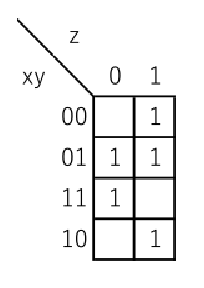
\includegraphics[width=3cm]{K_map2.eps}
                  \caption{$f_2$のカルノー図}
                  \label{fig:a2}
              \end{figure}
              この図から論理式$f_2$を簡略化すると
              \begin{align}
                  f_2 = \overline{x}z + y\overline{z} + \overline{y}z
              \end{align}
              となる。

          \end{description}
          \item [(b)]
          \begin{description}
              \item [$\rm \hspace{.08em}i\hspace{.08em}$.]
              まず、キューブ表現における1の個数ごとに最小項をグループ化し、変数消去の第1段階の表を以下の表\ref{tab:b1}にまとめた
              \begin{table}[H]
                  \caption{第1段階の表}
                  \label{tab:b1}
                  \centering
                  \begin{tabular}{|c|c|c|} \hline
                      キューブ表現 & 10進表現 & チェック  \\ \hline
                      001 & 1 & \\
                      010 & 2 & \\
                      100 & 4 & \\ \hline
                  \end{tabular}
              \end{table}
              この表から分かるように、論理式$f_1$は元々これ以上簡略化できない形で表されている。よって
              \begin{align}
                  f_1 = x\overline{yz} + \overline{x}y\overline{z} + \overline{xy}z
              \end{align}
              となる。

              \item [$\rm \hspace{.08em}ii\hspace{.08em}$.]
              まず、変数消去の第1,第2段階の表を以下の表\ref{tab:b2_1}\ref{tab:b2_2}にまとめた。
              \begin{table}[H]
                  \centering
                  \caption{第1段階の表}
                  \label{tab:b2_1}
                  \begin{tabular}{|c|c|c|} \hline
                      キューブ表現 & 10進表現 & チェック  \\ \hline
                      001 & 1 & \checkmark \\
                      010 & 2 & \checkmark \\
                      011 & 3 & \checkmark \\
                      101 & 5 & \checkmark \\
                      110 & 6 & \checkmark \\ \hline
                  \end{tabular}
              \end{table}
              \begin{table}[H]
                  \centering
                  \caption{第2段階の表}
                  \label{tab:b2_2}
                  \begin{tabular}{|c|c|c|} \hline
                      キューブ表現 & 10進表現 & チェック  \\ \hline
                      0-1 & {1, 3} &  \\
                      01- & {2, 3} &  \\
                      -01 & {1, 5} &  \\
                      -10 & {2, 6} &  \\ \hline
                  \end{tabular}
              \end{table}
              これらの表から主項表を作成し、表\ref{tab:b2_3}にまとめた。
              \begin{table}[H]
                  \centering
                  \caption{$f_2$の主項表}
                  \label{tab:b2_3}
                  \begin{tabular}{|c|c|c|c|c|c|} \hline
                      & 1 & 2 & 3 & 5 & 6 \\ \hline
                      $\overline{x}z\,(1,3)$ & \checkmark & & \checkmark & & \\ \hline
                      $\overline{x}y\,(2,3)$ & & \checkmark & \checkmark & & \\ \hline
                      $\overline{y}z\,(1,5)$ & \checkmark & & & \checkmark & \\ \hline
                      $y\overline{z}\,(2,6)$ & & \checkmark & & & \checkmark \\ \hline
                  \end{tabular}
              \end{table}
              この表から必要な項は$\overline{x}z\, , \, y\overline{z}\, , \,\overline{y}z$と分かる。
              よって、論理式$f_2$を簡略化すると
              \begin{align}
                  f_2 = \overline{x}z + y\overline{z} + \overline{y}z
              \end{align}
              となる。
          \end{description}

          \item [(c)]
          まず、論理変数の種類数が$n$で、キューブ表現における1の個数が$k$の時の最小項の数は、最大で
          \begin{align}
              \binom{n}{k}
          \end{align}
          と表される。
          更にここで、変数消去が進み$-$が$l$個ある場合の項の数は、最大で
          \begin{align}
              \binom{n}{l}\cdot\binom{n-l}{k} = \binom{n}{k} \cdot \frac{1}{l!}
          \end{align}
          と表される。
          ここから、比較回数として計算しなければいけないのは$-$の個数が$0$から$n-1$個のときまでなので、最大数は
          \begin{align}
              \sum_{l=0}^{n-1}\sum_{k=0}^{n-1}\left(\frac{1}{l!}\right)^2\binom{n}{k}\binom{n}{k+1}
          \end{align}
          と表され、$n$が大きくなると実用的ではないのが分かる。

      \end{description}
      \item [問3.]
      \begin{description}
          \item [(a)]
          まず、NAND,NORは論理的完全系であることは既知の事実とする。
          ここで\{AND,NOT\}と\{OR,NOT\}について考える。
          \{AND,NOT\}はそれぞれ組み合わせることでNANDを作ることができる。このときNANDは論理的完全系なので、\{AND,NOT\}も論理的完全系である。
          同様に、\{OR,NOT\}も組み合わせることでNORを作ることができる。このときNORは論理的完全系なので、\{OR,NOT\}も論理的完全系である。

          \item [(b)]
          一つ上げるとすれば\{1,AND,XOR\}がある。NOTは1と入力をXORにかけることで表す事ができる。ANDは含まれている。ORは一度XORに入力したものと、一度ANDに入力したものを再びXORに入力することで表す事ができる。よって、\{1,AND,XOR\}は論理的完全系の一つの組である。

          \item [(c)]
          XNORをNANDで表した回路図を図\ref{fig:3c}に表した。
          \begin{figure}[H]
              \centering
              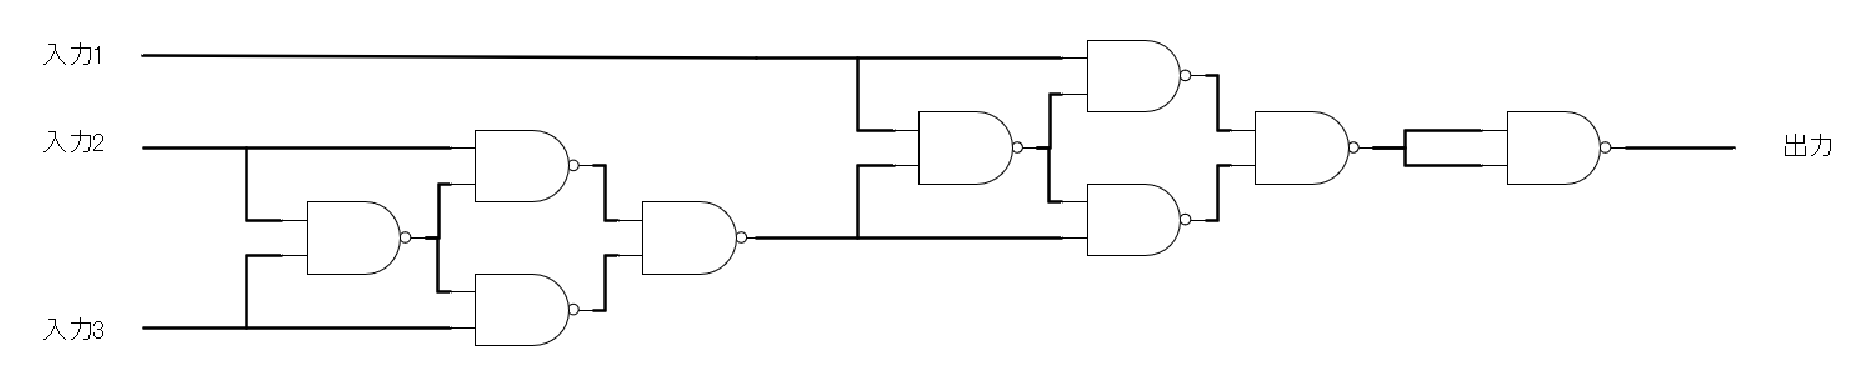
\includegraphics[width=10cm]{logic_3c.eps}
              \caption{XNORをNANDで表した回路図}
              \label{fig:3c}
          \end{figure}

          \item [(d)]
          \begin{description}
              \item [$\rm \hspace{.08em}i\hspace{.08em}$.]
              論理式$f_1$をNORで表した回路図を図\ref{fig:3d_1}に表した
              \begin{figure}[H]
                  \centering
                  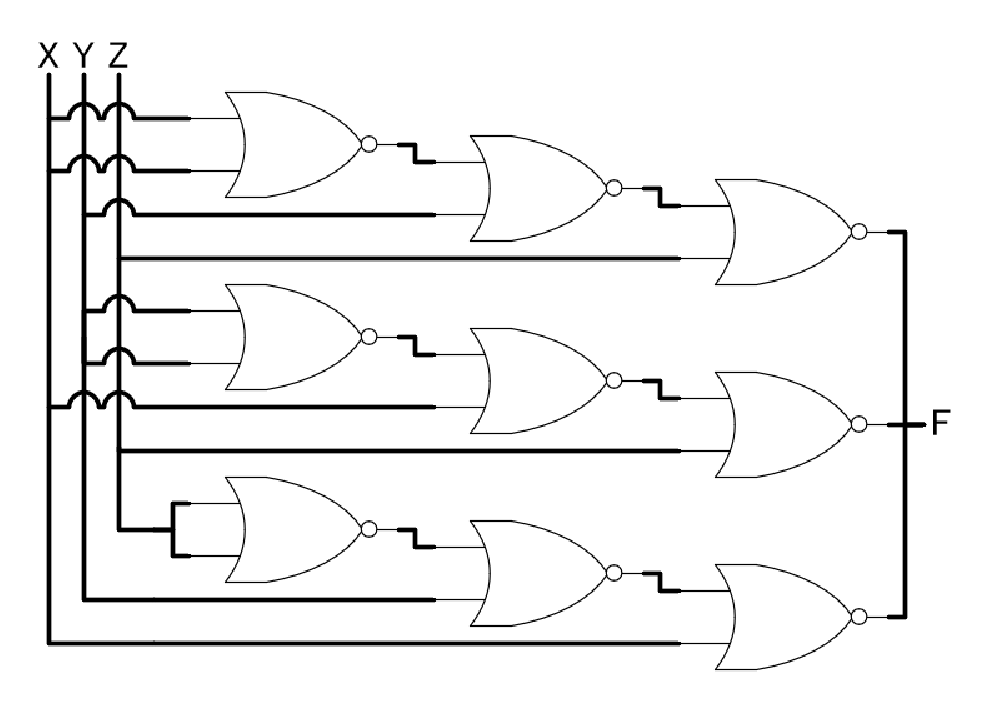
\includegraphics[width=8cm]{logic_3d_1.eps}
                  \caption{$f_1$をNANDで表した回路図}
                  \label{fig:3d_1}
              \end{figure}

              \item [$\rm \hspace{.08em}ii\hspace{.08em}$.]
              論理式$f_2$をNORで表した回路図を図\ref{fig:3d_2}に表した
              \begin{figure}[H]
                  \centering
                  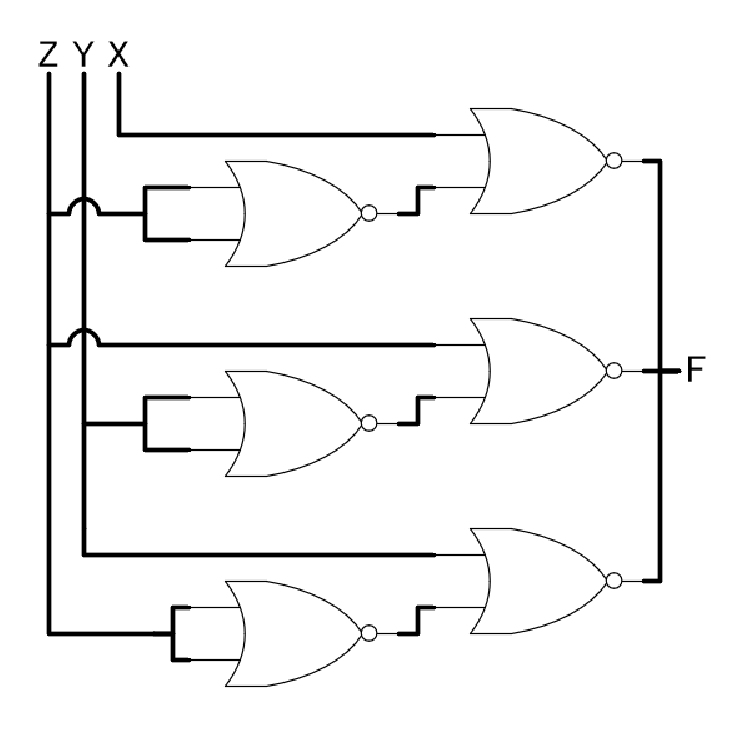
\includegraphics[width=6cm]{logic_3d_2.eps}
                  \caption{$f_2$をNANDで表した回路図}
                  \label{fig:3d_2}
              \end{figure}

          \end{description}
      \end{description}
      \item [問4.]
      2進数の入力に1を加算した結果を出力する組み合わせ回路を作成し、図\ref{fig:4}に記した。
      \begin{figure}[H]
          \centering
          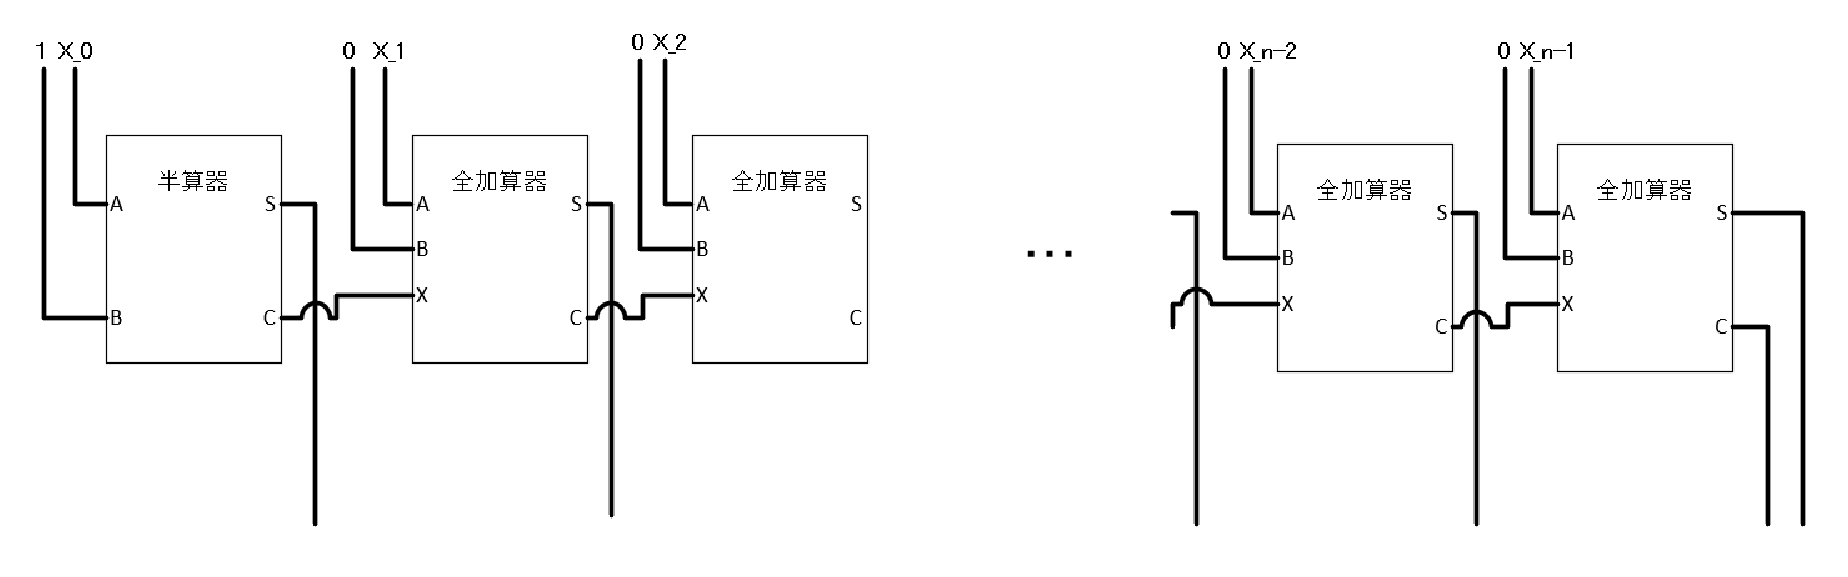
\includegraphics[width=10cm]{logic_4.eps}
          \caption{1を加算した結果を出力する回路図}
          \label{fig:4}
      \end{figure}
  \end{description}
\end{document}
